% ----------------------------------------------------------------------
% Unofficial UCLA SCC Latex Beamer Presentation
% Author: Denise Ferrari  <denise@stat.ucla.edu>
% Date: 03/17/2009
% ----------------------------------------------------------------------
% This presentation requires the following files:
%
% beamerthemeSCC.sty
% beamerouterthemeSCC.sty
% beamercolorthemeSCC.sty
% logo.png
% ----------------------------------------------------------------------
% ----------------------------------------------------------------------

\documentclass[11pt]{beamer}

%% To get handouts:
% \documentclass[11pt,containsverbatim,handout]{beamer}

%% include when making handouts
% \usepackage{pgfpages}
% \pgfpagesuselayout{4 on 1}[letterpaper,landscape,border shrink=5mm]

% *****************************************
% Theme
% *****************************************

% use compress for circles to be on one line
% o/w take it out
% \usetheme{SCC}
\usetheme[compress]{SCC}

% *****************************************
% Packages
% *****************************************
\usepackage{graphicx}
\usepackage{amssymb}
\usepackage{epstopdf}
\usepackage{listings}
\usepackage{hyperref}
\usepackage{color}

\DeclareGraphicsRule{.tif}{png}{.png}{`convert #1 `dirname #1`/`basename #1 .tif`.png}

\lstloadlanguages{R} 
\lstset{language=R,%
basicstyle=\small\ttfamily,%
stringstyle=\color{magenta},%
showstringspaces=false,%
keywordstyle=\color{red}\mdseries\underbar,%
commentstyle=\color{blue}\textsl,%
xleftmargin=4ex,%
numbers=left,%
numberstyle=\tiny,%
stepnumber=1,%
firstnumber=1,%
breaklines=true%
}

% *****************************************
% New Commands
% *****************************************
\newcommand{\urlwofont}[1]
{
\urlstyle{same}\url{#1}
}

% Presentation

\begin{document}
	% Title
% Note: [short title]{long title}, [short author(s) name]{long author(s) name}
\title{ Introduction to Visualizations with \ttfamily R \normalfont }
%\subtitle{}
\author{Irina Kukuyeva, Ph.D. \\ \ttfamily \url{www.KukuyevaConsulting.com} \normalfont}
%\institute[UCLA SCC]{UCLA Extension Track 1\\UCLA Department of Statistics \\ Statistical Consulting Center}
\date{March 3, 2016}



% Title Frame 
\frame{ \titlepage }

	% TOC
\begin{frame}[shrink=6]
	\frametitle{Outline}
	\tableofcontents[hideallsubsections]
\end{frame}

% Before any section, show a slide that highlights the current section 
\AtBeginSection[]
{
	\begin{frame} [shrink=6]
		\tableofcontents[currentsection,hideothersubsections]
	\end{frame}
}
	%%%%%%%%%%%%%%%%%%%%%%%%%%%%%%%%%%%%%

%%%%% Disclaimer
%\normalfont
%\begin{frame}
%	\begin{center}
%  		\begin{block}{Disclaimer} 
%The author assumes you know the theory behind Box-Jenkins time series models. \\
%This tutorial will teach you how to apply what you have learned, using R.
%		\end{block}
%	\end{center} 
%\end{frame}

%%%%%%%%%%%%%%%%%%%%%%%%%%%%%%%%%%%%%

%%%%%%%%%%%%%%%%%%%%%%%%%%%%%%%%%%%%%

% Section: Preliminaries

\section[Prelim]{Preliminaries}

% Subsection: Software Installation

\subsection{Software Installation}

%%%%%%%%%%%%%%%%%%%%%%%%%%%%%%%%%%%%%

\begin{frame}
\frametitle{Installing R on a Mac}

\begin{columns}
\column{0.50\textwidth}
\begin{enumerate}
\item Go to \small \ttfamily http://cran.r-project.org/ \normalfont \normalsize and select \itshape MacOS X \normalfont
\item Select to download the latest version: 2.9.1 (2009-06-26)
\item Install and Open.  The R window should look like this:
\end{enumerate}
%
\column{0.50\textwidth}
\begin{center}
\includegraphics[width=1\textwidth]{images/Rwindow}
\end{center}
\end{columns}

\end{frame}

%%%%%%%%%%%%%%%%%%%%%%%%%%%%%%%%%%%%%

% Subsection: R Help

\subsection{R Help}

%%%%%%%%%%%%%%%%%%%%%%%%%%%%%%%%%%%%%
\begin{frame}[fragile]
\frametitle{R Help}

\begin{columns}
\column{0.4\textwidth}
For help with any function in R, put a question mark before the function name to determine what arguments to use, examples and background information.

\begin{lstlisting}
?plot
\end{lstlisting}

\column{0.6\textwidth}
\begin{center}
\includegraphics[width=1.1\textwidth]{images/help}
\end{center}
\end{columns}

\end{frame}

%%%%%%%%%%%%%%%%%%%%%%%%%%%%%%%%%%%%%

% Subsection: Importing Data Sets into R

\subsection[Importing Data]{Importing Data Sets into R}

%%% Subsection: Importing Data from the Internet

\subsubsection{Importing Data from the Internet}

%%%%%%%%%%%%%%%%%%%%%%%%%%%%%%%%%%%%%
% --------------------------------------------------- Slide --
\begin{frame}[fragile]
  \frametitle{Data from the Internet}

 When downloading data from the internet, use \ttfamily read.table(). \normalfont  In the arguments of the function:
   \begin{itemize}
   \item \ttfamily header: \normalfont if TRUE, tells R to include variables names when importing
   \item \ttfamily sep: \normalfont tells R how the entires in the data set are separated
     \begin{itemize}
       \item \ttfamily sep=",": \normalfont when entries are separated by COMMAS
       \item \ttfamily sep="$\backslash t$": \normalfont when entries are separated by TAB
       \item \ttfamily sep=" ": \normalfont when entries are separated by SPACE
     \end{itemize}
    \end{itemize}
    	\begin{lstlisting}
data<-read.table("http://www.stat.ucla.edu
/~vlew/stat130a/datasets/twins.csv", 
header=TRUE, sep=",")
	\end{lstlisting}
\normalfont
\normalsize
\end{frame}

%%%%%%%%%%%%%%%%%%%%%%%%%%%%%%%%%%%%%

% Data from your Computer

\subsubsection{Importing Data from Your Computer}

%%%%%%%%%%%%%%%%%%%%%%%%%%%%%%%%%%%%%
\begin{frame}[fragile]
 \frametitle{Importing Data from Your Computer}
     \begin{enumerate}
  	\item Check what folder R is working with now: \\
		\begin{lstlisting}
getwd()
		\end{lstlisting}

  	\item Tell R in what folder the data set is stored (if different from (1)).  Suppose your data set is on your desktop: \\
	\begin{lstlisting}
setwd("~/Desktop")
	\end{lstlisting}

	\item Now use the \ttfamily read.table() \normalfont command to read in the data, substituting the name of the file for the website.
     \end{enumerate}
\end{frame}

%%%%%%%%%%%%%%%%%%%%%%%%%%%%%%%%%%%%%

% Data Available in R
\subsubsection{Using Data Available in R}

%%%%%%%%%%%%%%%%%%%%%%%%%%%%%%%%%%%%%
\begin{frame}[fragile]
  \frametitle{Using Data Available in R}
\begin{enumerate}
\item To use a data set available in one of the R packages, install that package (if needed).

\item Load the package into R, using the \ttfamily library() \normalfont function. \\
	\begin{lstlisting}
library(alr3)
	\end{lstlisting}

\item Extract the data set you want from that package, using the \ttfamily data() \normalfont function.  In our case, the data set is called \ttfamily UN2. \\
	\begin{lstlisting}
data(UN2)
	\end{lstlisting}

\end{enumerate}
\end{frame}


	\part{Visualizations}

% ------------------------------------------------------------
% ------------------------------------------------------------
\section{Data Set}
\begin{frame}[allowframebreaks, fragile]
	% data <- read.csv("../data/Number_of_Selected_Inpatient_Medical_Procedures__California_Hospitals__2005-2014.csv")
\end{frame}


% ------------------------------------------------------------
% ------------------------------------------------------------
\section[Summary Plots]{Summary Plots}

\subsection{Scatterplot}
%%%%% New frame
\begin{frame}[allowframebreaks, fragile]
\frametitle{Scatterplot (v0.1)}
  \framesubtitle{Data = CA ???}

To get a quick peak into the numerical variables in the data \ttfamily scatterplotMatrix(): \normalfont
  		\begin{lstlisting}[ basicstyle=\small ]
# Load package `car' to use scatterplotMatrix():	
### Summary plots 
library(car)	
scatterplotMatrix(
	x = data[, c("Latitude", "Longitude", "Volume")], 
	smoother = FALSE, 
	reg.line = FALSE
	)
		\end{lstlisting}
% col=rgb(0.4, 0.2, 0.2, alpha=0.5)

        \begin{center}
         \includegraphics[width=0.63\textwidth]{images/scatterPlot_v0.pdf}
        \end{center}
\end{frame}

\begin{frame}[allowframebreaks, fragile]
\frametitle{Scatterplot (v0.2)}

To get a quick peak into the numerical variables and the trends in the data, modify arguments of \ttfamily scatterplotMatrix(): \normalfont
  		\begin{lstlisting}
?scatterplotMatrix # for documentation
library(car)		
scatterplotMatrix(
	x = data[, c("Latitude", "Longitude", "Volume")], 
	reg.line = FALSE
	)
		\end{lstlisting}

        \begin{center}
         \includegraphics[width=0.63\textwidth]{images/scatterPlot_v1.pdf}
        \end{center}
\end{frame}

\begin{frame}[allowframebreaks, fragile]
\frametitle{Scatterplot (v0.3)}

To improve the color scheme, modify arguments of \ttfamily scatterplotMatrix().  
  		\begin{lstlisting}[ basicstyle=\tiny]
library(car)		
scatterplotMatrix(
	x = data[, c("Latitude", "Longitude", "Volume")], 
	reg.line = FALSE,
	col=c(3,
		"orangered",
		rgb(176/256, 196/256, 222/256, alpha=0.5)
		), 
	pch=19,
	lwd=3
	)
		\end{lstlisting}
\normalfont
\framebreak
You can specify a color in R via: 
\begin{itemize}
	\item Number (e.g. 1 = black, 2 = red, etc.)
	\item Name (e.g. "black", "red", "dodgerblue")
	\item RGB (e.g. c(0,0,0) = black, c(1,0,0) = red, etc.)
	\item Please see \url{http://research.stowers-institute.org/efg/R/Color/Chart/} for color references. 
\end{itemize}

\noindent Note the order of color arguments. \normalfont
        \begin{center}
         \includegraphics[width=0.63\textwidth]{images/scatterPlot_v3.pdf}
        \end{center}
\end{frame}

%---
\begin{frame}[allowframebreaks, fragile]
\frametitle{Scatterplot (v0.4)}
  \framesubtitle{Data = Fiji Earthquakes Since 1964}

Another way to get a quick peak into the numerical variables in the data is via \ttfamily ggpairs(): \normalfont
  		\begin{lstlisting}[ basicstyle=\small ]
library(ggplot2)
library(GGally)
ggpairs(
	data[, c("Latitude", "Longitude", "Volume")]
	)
		\end{lstlisting}
% col=rgb(0.4, 0.2, 0.2, alpha=0.5)

        \begin{center}
         \includegraphics[width=0.6\textwidth]{images/scatterPlot_v4.pdf}
        \end{center}
\end{frame}

%%%%% New frame
\subsection{Histogram}
\begin{frame}[fragile, allowframebreaks]
\frametitle{'Nicer' Histogram (v0.1)}
  \framesubtitle{Data = Tooth Growth of Guinea Pigs}

To compare the frequencies of two variables side-by-side, use \ttfamily beanplot(): \normalfont

	\begin{lstlisting}[ basicstyle=\tiny ]
library(beanplot)
op <- par(las=2)
beanplot(
	Volume ~ as.factor(County), 
	data = data_LA_SF, 
	xlab = "",
	log = "y",
	side = "both", 
	col = list( c( grey(0.5), "white"), grey(0.8) ), 
	border = NA, 
	overallline = "median", 
	ll = 0.005
	)
legend(
	x = "bottomleft",
	fill=c( grey(0.5), grey(0.8) ), 
	legend=c( "LA", "SF" )
	)
par(op)
	\end{lstlisting}

        \begin{center}
	         \includegraphics[width=0.65\textwidth]{images/beanplot_v0.pdf}
        \end{center}

\end{frame}


%%% NOT WORK...
%
%library(lattice)
%split.screen(c(1,2))        # split display into two screens
%split.screen(c(2,1),2)      # split bottom half in two
%screen(1)                   # prepare screen 1 for output
%qqplot(ToothGrowth$len~ToothGrowth$supp)
%screen(4)                   # prepare screen 4 for output
% # boxplot(ToothGrowth$len~ToothGrowth$supp)
% beanplot(ToothGrowth$len~ToothGrowth$supp, col=list(grey(0.5),c(grey(0.8),"white")), border = NA, overallline = "median", ll=0.01, side="both")
%screen(1, FALSE)            # return to screen 1, but do not clear
%close.screen(all = TRUE)    # exit split-screen mode


%%%%%%%%%%%%%%%%%%%%%%%%%%%%%%%%%%%%%

% ------------------------------------------------------------
% ------------------------------------------------------------

% Exercise: compare distributions of Iris data
% ID outlier in dataset

\subsection{Exercise I}
\begin{frame}
	\frametitle{Exercise I}
	Compare the distributions of the sepal widths for the three species of irises (using the \ttfamily iris \normalfont data set).
\end{frame}
		% pie chart, histogram
	% http://www.r-bloggers.com/time-series-plots-in-r/
% http://www.fromthebottomoftheheap.net/2013/10/23/time-series-plots-with-lattice-and-ggplot/


% ------------------------------------------------------------
% ------------------------------------------------------------

%%%%%%%%%%%%%%%%%%%%%%%%%%%%%%%%%%%%%

% Section: Plots of TS in R 

\section[Time Series Plots]{Time Series Plots}
%%%%%%%%%%%%%%%%%%%%%%%%%%%%%%%%%%%%%

%\subsection{Univariate Plots}
%%%%%%%%%%%%%%%%%%%%%%%%%%%%%%%%%%%%%%

%\begin{frame}[fragile]
% \frametitle{Univariate Time Series Plot  \footnote{This section is from the SCC Mini-Course "Introductory Time Series \\ with R" by Irina Kukuyeva}}

%To plot one variables one at a time, use \ttfamily plot(): \normalfont 
%    \begin{columns}
%      \column{0.55\textwidth}
%		\begin{lstlisting}
%data(EuStockMarkets)
%dax<-EuStockMarkets[, 1]
%plot(dax)
%		\end{lstlisting}

%      \column{0.45\textwidth}
%       \begin{center}
%         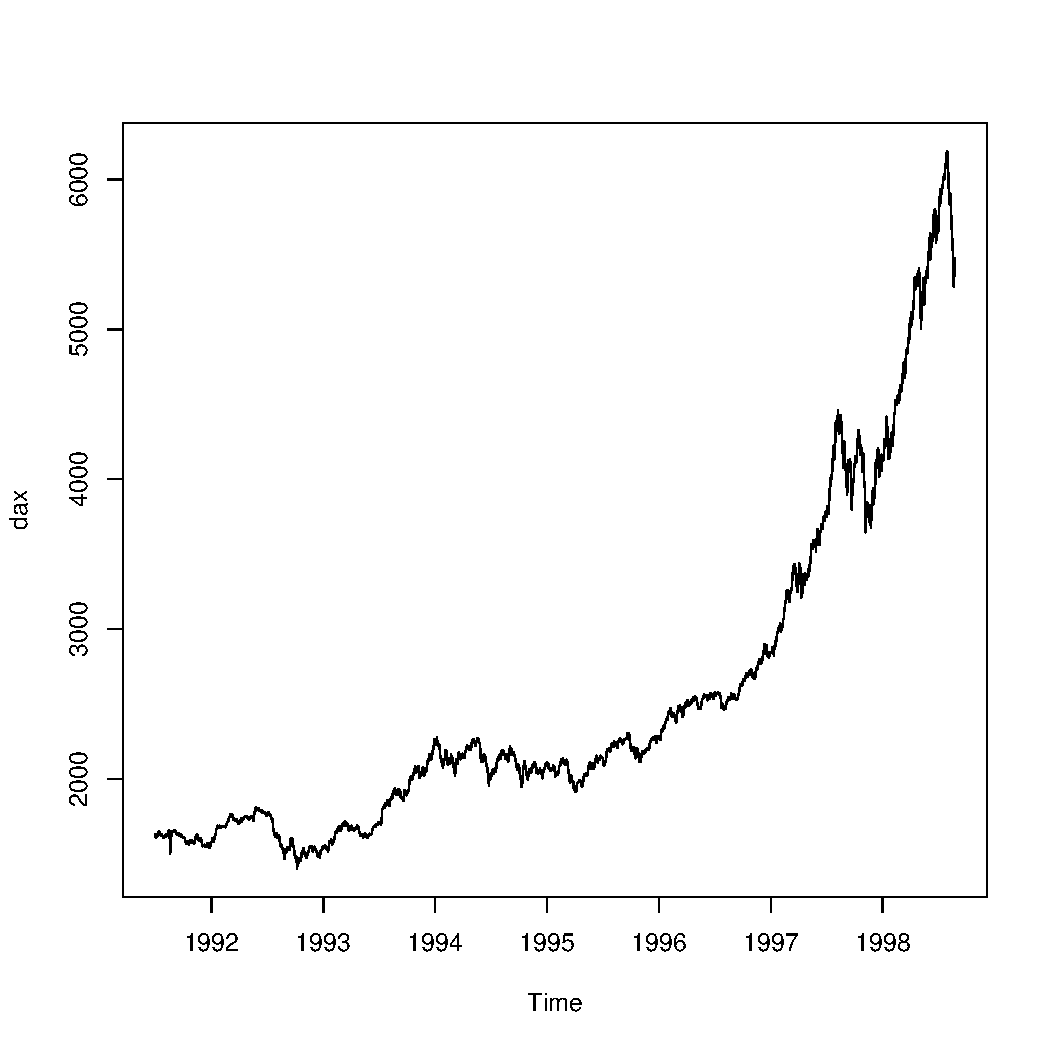
\includegraphics[width=0.95\textwidth]{images/daxPlot.pdf}
%        \end{center}
%      \end{columns}

%\end{frame}

%%%%%%% New frame
%\begin{frame}[allowframebreaks, fragile]
% \frametitle{Customizing the plot}

%To plot more than variables one at a time, use \ttfamily xyplot(): \normalfont
%		\begin{lstlisting}
%# After processing data as in Approach 1
%# load both libraries:
%library(lattice)
%library(zoo)
%data(EuStockMarkets)
%z<-EuStockMarkets
%xyplot(z, screen = c(1,1,1,1), col = 1:4, strip = FALSE)
%legend(1992, 5000, colnames(z), lty = 1, col = 1:4)
%		\end{lstlisting}

%       \begin{center}
%         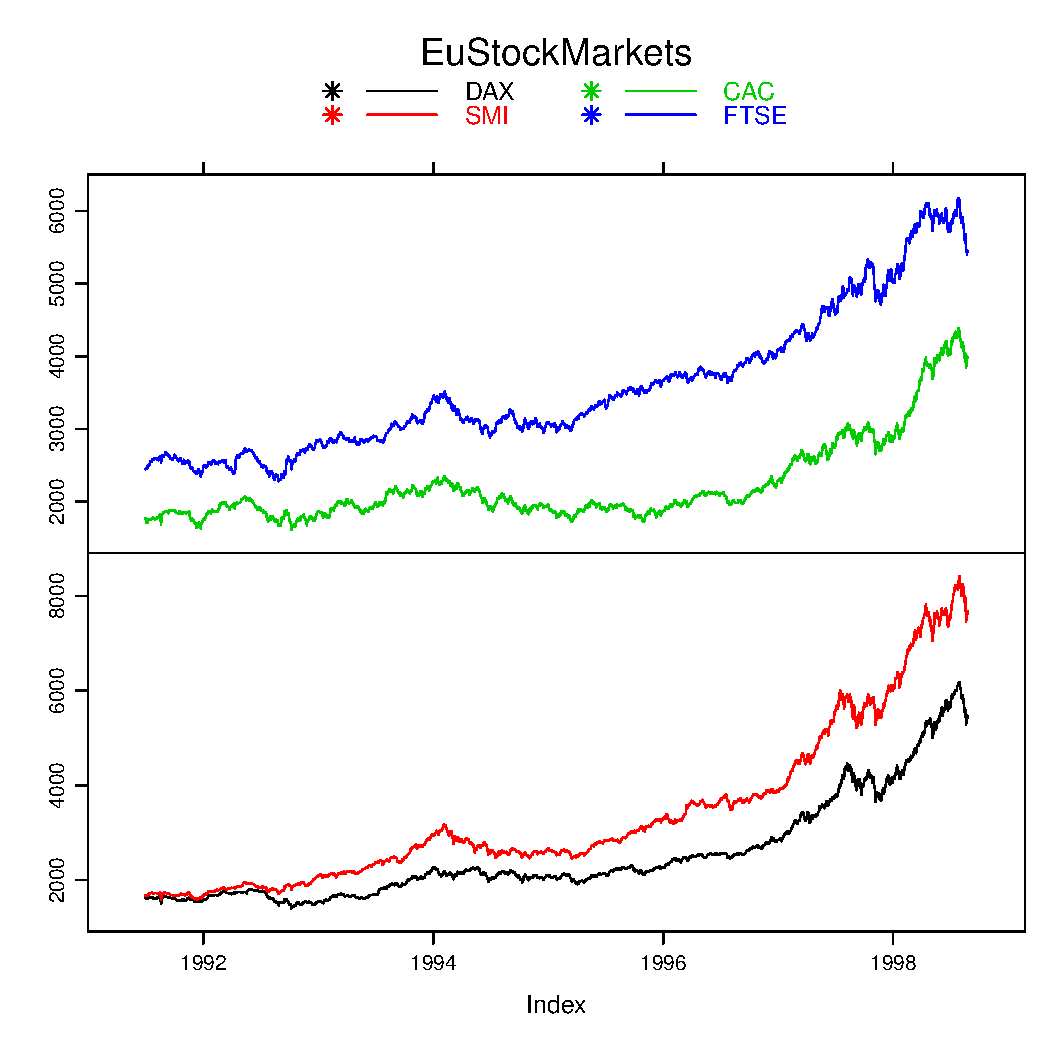
\includegraphics[width=0.85\textwidth]{images/stockPlot2}
%        \end{center}
%\end{frame}

%%%%%%%%%%%%%%%%%%%%%%%%%%%%%%%%%%%%%

\subsection{Multivariate Plots}

%%%%%%%%%%%%%%%%%%%%%%%%%%%%%%%%%%%%%

\begin{frame}[allowframebreaks, fragile]
 \frametitle{Multivariate Plots: Approach 1}

To plot more than variables one at a time, use \ttfamily xyplot()\normalfont [5]:
%\begin{itemize}
%	\item For documentation, go to: www.jstatsoft.org/v25/c01/paper 
%	\item Go to: http://www.biostat.jhsph.edu/$\sim$rpeng/RR/mvtsplot/
%	\item Copy the relevant R Code and paste it into the R Console. Press ENTER.
%	\item Plot your data
% \end{itemize}
		\begin{lstlisting}
### Step 0: Load any required packages:
library(dplyr)
library(lattice)

### Step 1: Get data for one procedure:
df_LA_CABG <- df %>%
  filter( 
    (County == "Los Angeles") & 
    (Procedure == "CABG") & 
    (Volume > 0) 
    )
    \end{lstlisting}

\newpage    
    \begin{lstlisting}
### Step 2: Visualize    
xyplot( Volume ~ Year | Hospital.Name, 
  data=df_LA_CABG,
  par.strip.text=list(cex=0.5),
  type="b",
  main="LA Coronary artery bypass grafting (CABG)"
  )
		\end{lstlisting}

\newpage
      \vspace{-20pt} \hspace{-20pt}
         \includegraphics[width=1.05\textwidth]{images/timeseries_LA_CABG}

\end{frame}

%---
\begin{frame}[fragile, allowframebreaks]
 \frametitle{Multivariate Plots: Approach 2}

Another way to plot more than one variable at a time, is via \ttfamily ggplot()\normalfont :

    \begin{lstlisting}
### Step 0: Load any required packages:
library(dplyr)
library(ggplot2)

### Step 1: Get data for one hospital:
df_Cedars <- df_clean %>%
  filter( Hospital.Name == 'Cedars Sinai Medical Center')
   \end{lstlisting}

\newpage
    \begin{lstlisting}
### Step 2: Visualize
ggplot( data = df_Cedars ) + 
  geom_line( aes(
    x = Year, 
    y = Volume, 
    linetype = Procedure) ) +
  scale_x_continuous( breaks=seq(
    from=2005, 
    to=2014, 
    by=3) ) +
  theme_classic() +
  ggtitle( "Volume of Procedures for Cedars Sinai Medical Center" )
   \end{lstlisting}

\newpage
       \begin{center}
         \includegraphics[width=0.9\textwidth]{images/timeseries_Cedars}
        \end{center}
\end{frame}

% % ------------------------------------------------------------
% % ------------------------------------------------------------
\subsection{Exercise II}
\begin{frame}[fragile]
	\frametitle{Exercise II}
	In the healthcare data set, what seems to be the most popular procedure in CA?\\
  \vspace{10pt}
  \noindent Hints: \small

    %%% TODO: show how to aggregate it by year and procedure

    \normalsize
\end{frame}

		% mtvsplot, plot, xyplot
		% changing plotting options
	
% ------------------------------------------------------------
% ------------------------------------------------------------

\section[Geo]{Geographical Plots}
%%%%%%%%%%%%%%%%%%%%%%%%%%%%%%%%%%%%%
\subsection{Maps}
%%%%%%%%%%%%%%%%%%%%%%%%%%%%%%%%%%%%%

\begin{frame}[fragile]
\frametitle{Geographic Maps}
  \framesubtitle{Map of Fiji Earthquakes Since 1964}

To overlay a map to a plot containing latitude and longitude, load the package \ttfamily maps: \normalfont 
    \begin{columns}
      \column{0.50\textwidth}
\begin{lstlisting}
data(quakes)
library(maps)
plot(quakes[, 2], quakes[, 1], xlim=c(100, 190), ylim=c(-40, 0))
map("world", add=T)
\end{lstlisting}

     \column{0.50\textwidth}
       \begin{center}
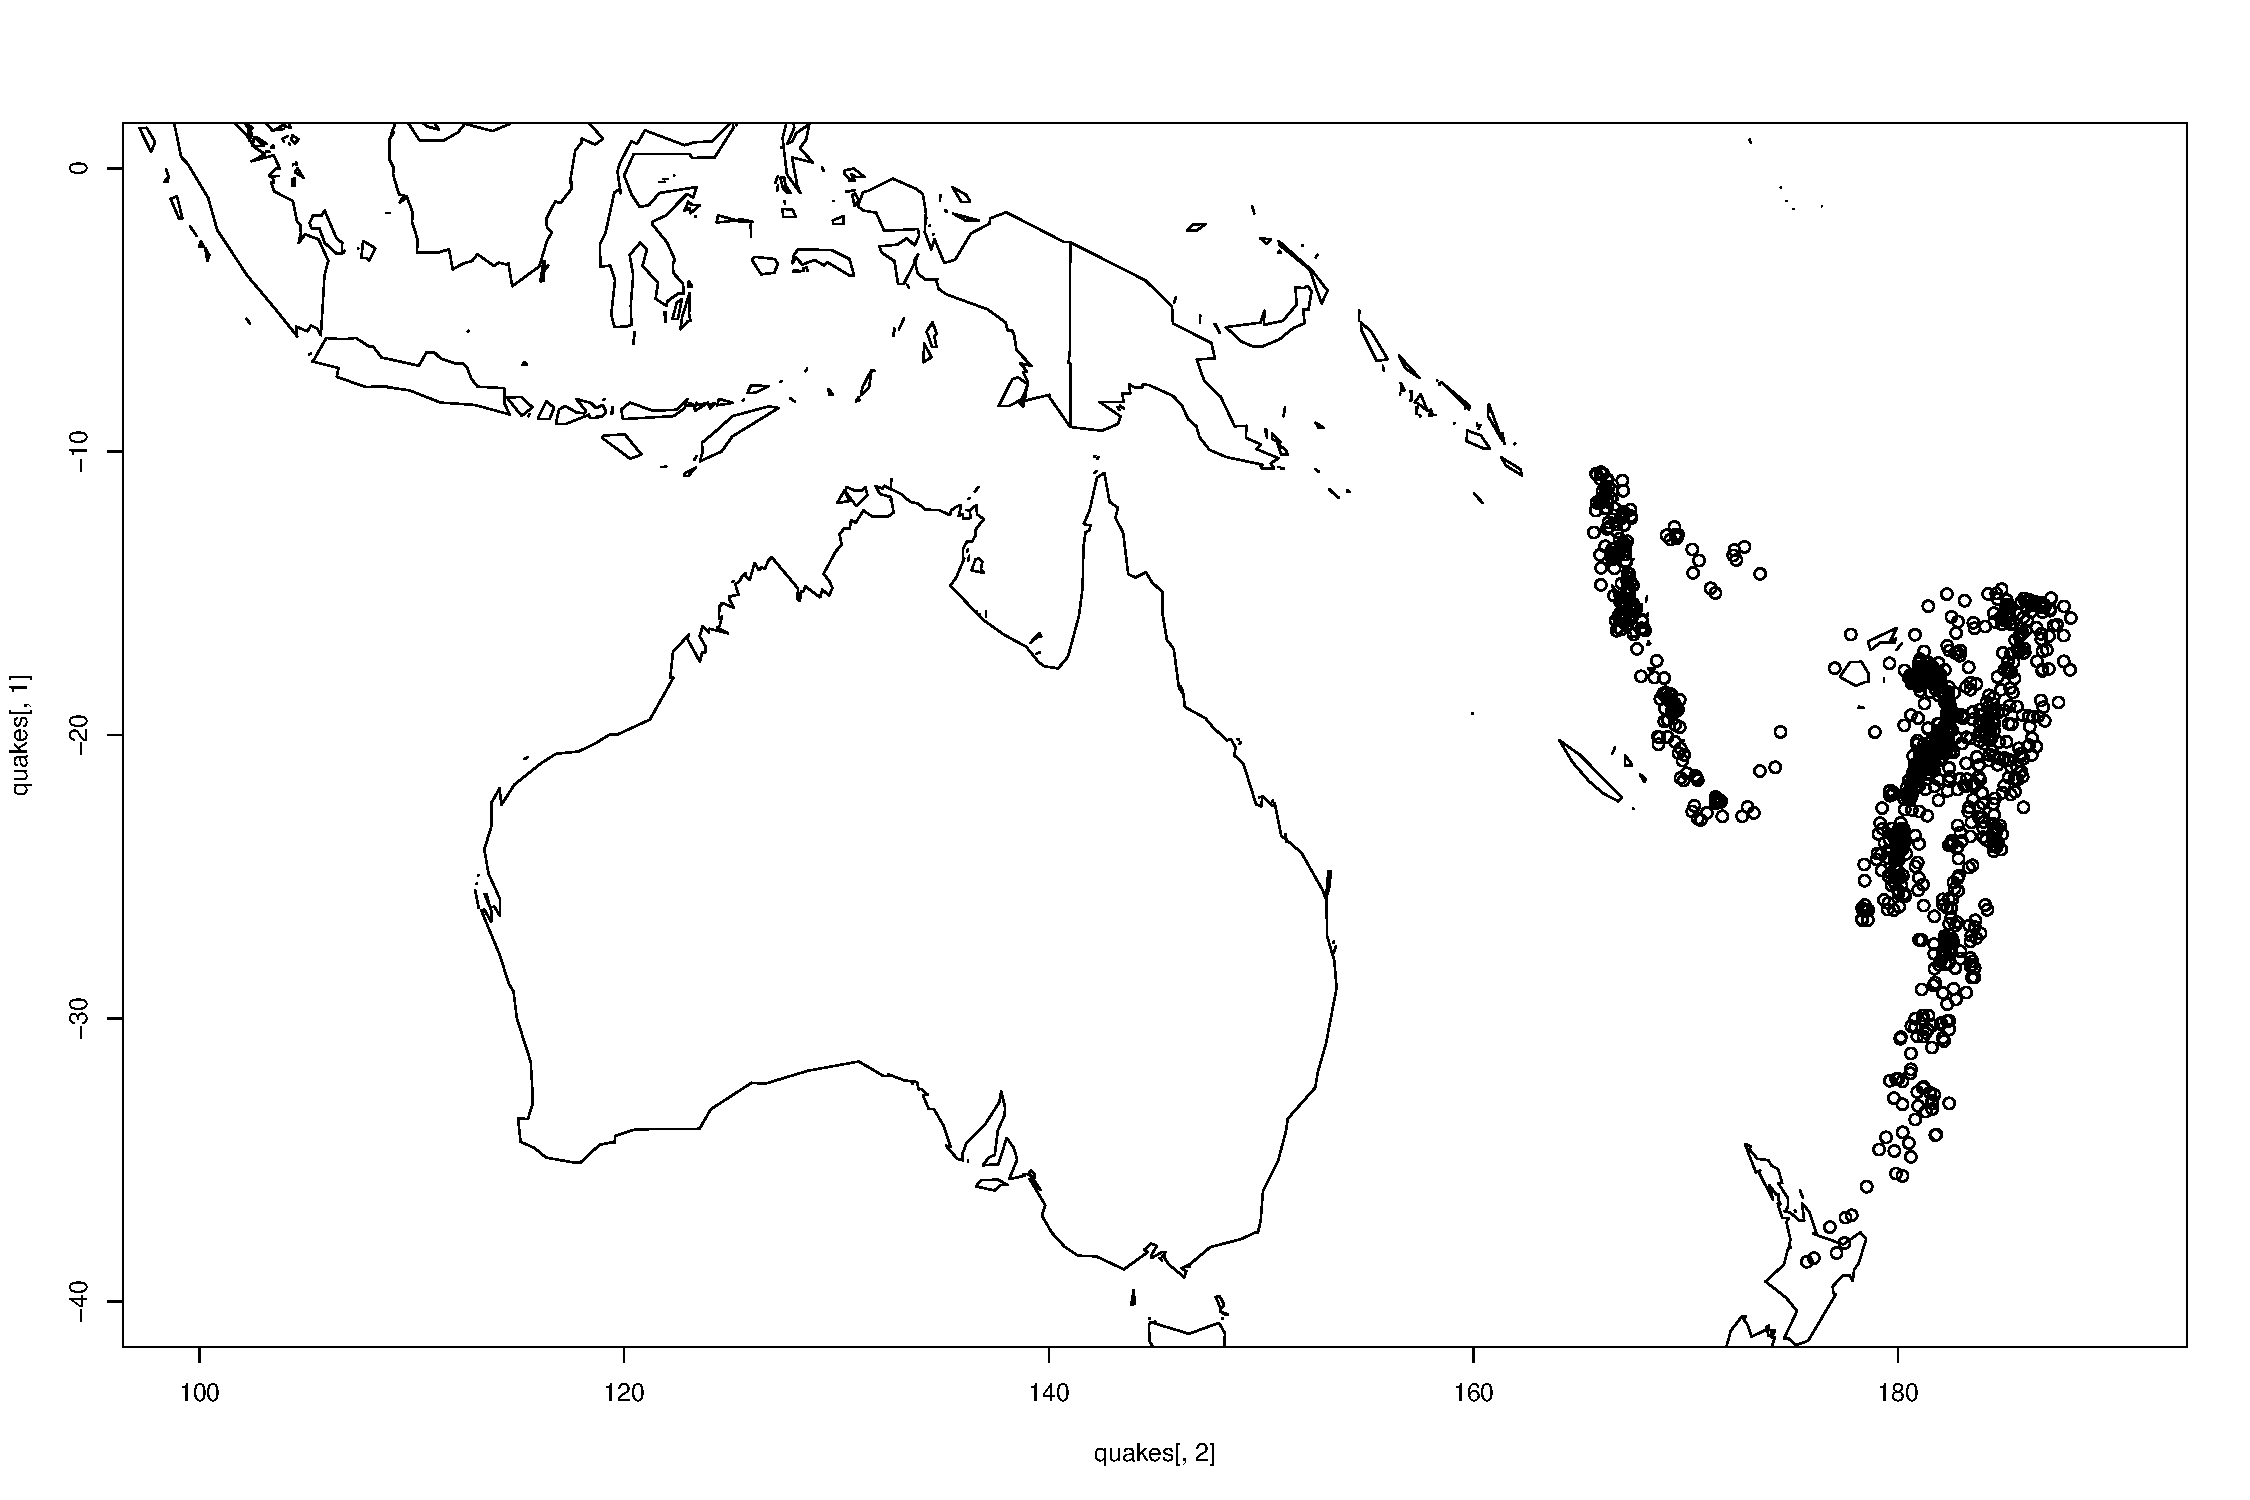
\includegraphics[width = 55mm]{images/Fuji.pdf}
\end{center}
\end{columns}
\end{frame}

%%%%%%%%%%%%%%%%%%%%%%%%%%%%%%%%%%%%%
\subsection{Projection Maps}
%%%%%%%%%%%%%%%%%%%%%%%%%%%%%%%%%%%%%

\begin{frame}[allowframebreaks, fragile]
\frametitle{Projection Maps}
  \framesubtitle{Map of Fiji Earthquakes Since 1964}

For a different perspective of a map, use  \ttfamily mapproject(): \normalfont 

\begin{lstlisting}
library(mapproj)
library(maps)
m <- map('world',plot=FALSE)
# Projection is Azimuthal with equal-area
map('world',proj='azequalarea',orient=c(longitude=0,latitude=180,rotation=0))
map.grid(m,col=2)
points(mapproject(list(y=quakes[which(quakes[, 4]>=6), 1],x=quakes[which(quakes[, 4]>=6), 2])),col="blue",pch="x",cex=2)
\end{lstlisting}

\newpage
       \begin{center}
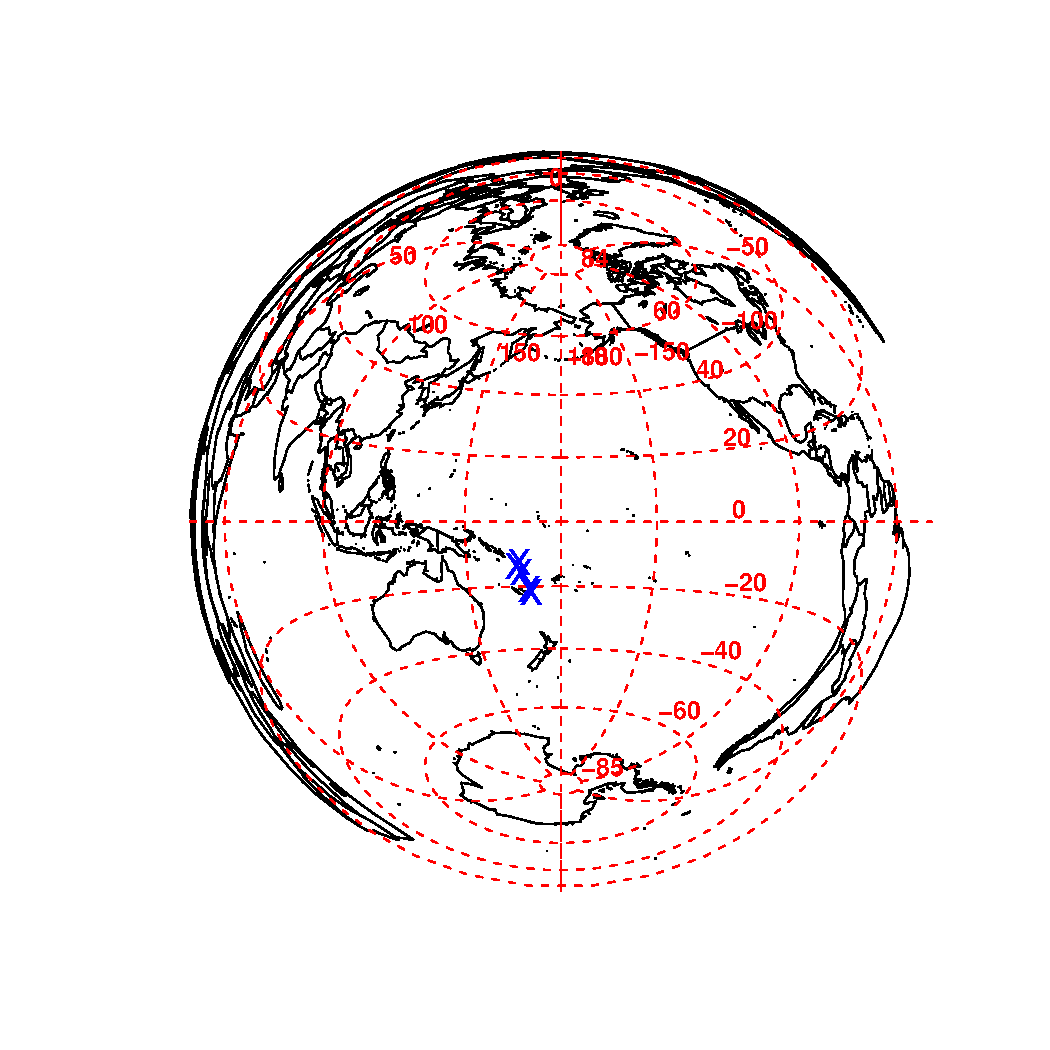
\includegraphics[width = 70mm]{images/Fuji2.pdf}
\end{center}

\end{frame}

%%%%%%%%%%%
\begin{frame}[fragile]
	\begin{alertblock}{Bonus Feature of the \ttfamily maps \normalfont package:}
		To determine in which part of the world the observations are (based on latitude and longitude), use \ttfamily map.where(): \normalfont
			\begin{lstlisting}		
				in.what.country<-map.where(database="world", quakes[, 2], quakes[, 1])
			\end{lstlisting}
		To determine which observations are in the ocean: \normalfont
			\begin{lstlisting}
				# Number of points in ocean after filtering:
				ind<-sum(is.na(in.what.country)); ind
				# Number of observations: 1000
				# Number in Ocean: 993
			\end{lstlisting}
	\end{alertblock}

\end{frame}

% ------------------------------------------------------------
% ------------------------------------------------------------

		% maps +points, bubbleplot
		% locator, identify
		% color-coding for intensity
	%
% ------------------------------------------------------------
% ------------------------------------------------------------

%%%%%%%%%%%%%%%%%%%%%%%%%%%%%%%%%%%%%
\section{3D Plots}
\subsection{\ttfamily lattice \normalfont library}

%%%%%%%%%%%%%%%%%%%%%%%
\begin{frame}[fragile]
\frametitle{3D Images with Package \ttfamily lattice \normalfont}

\vspace{0.1in}
\bf{Method 1:} \normalfont Using \ttfamily wireframe(): \normalfont 

    \begin{columns}
      \column{0.50\textwidth}
\begin{lstlisting}
library(lattice)
wireframe(volcano, col.regions = terrain.colors(100), asp = 1, color.key=TRUE, drape=TRUE, scales = list(arrows = FALSE))
\end{lstlisting}
%g <- expand.grid(x = 1:10, y = 5:15)
%g$z<-g$x^2
%wireframe(g$z~g$x*g$y, scales = list(arrows = FALSE), drape = TRUE, colorkey = TRUE)

     \column{0.50\textwidth}
       \begin{center}
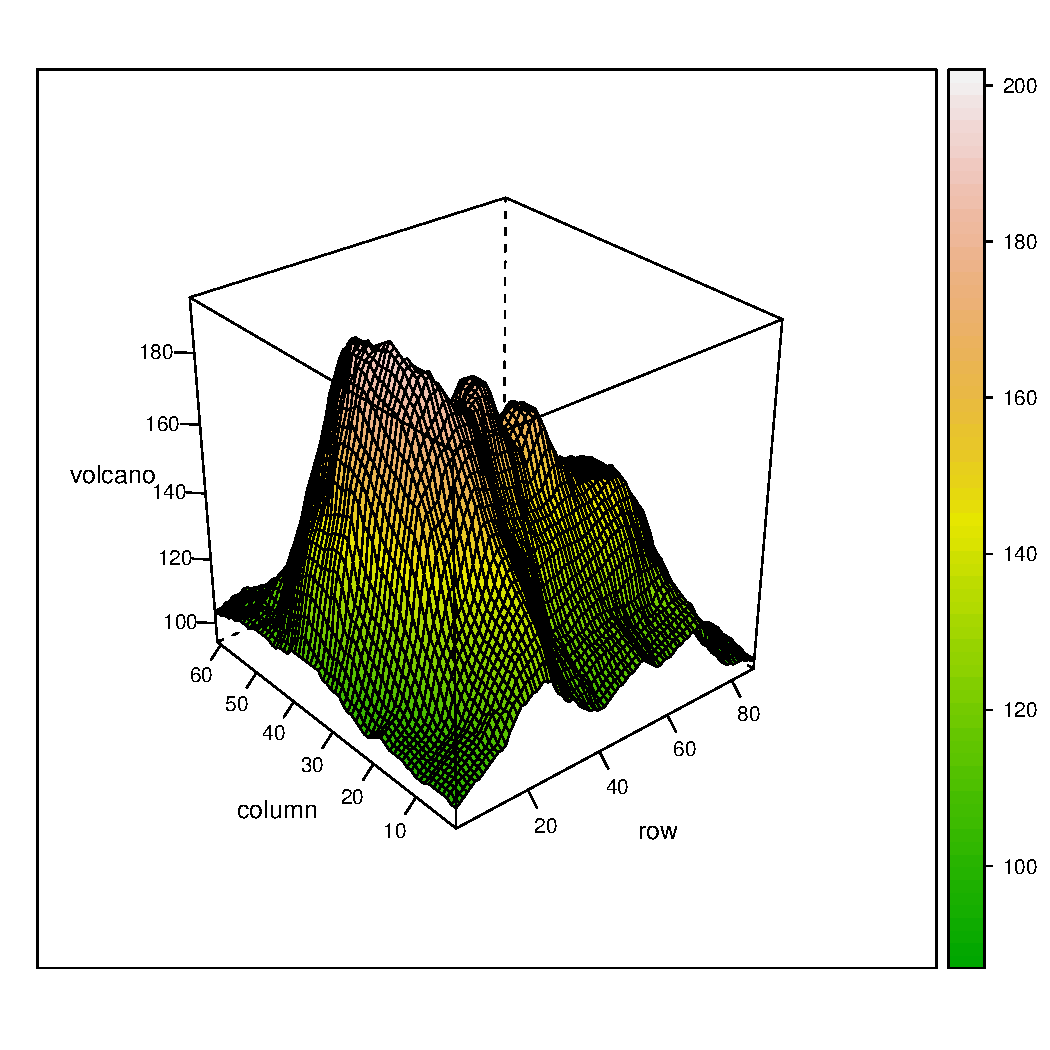
\includegraphics[width = 55mm]{images/wireframe.pdf}
\end{center}
\end{columns}
\end{frame}

%%%%%%%%%%%%%%%%%%%%%%%
\begin{frame}[fragile]
\frametitle{3D Images with Package \ttfamily lattice \normalfont}

\bf{Method 2:} \normalfont Same image with the \ttfamily levelplot() \normalfont function:

    \begin{columns}
      \column{0.50\textwidth}
\begin{lstlisting}
library(lattice)
levelplot(volcano, asp=1, col.regions=terrain.colors)
\end{lstlisting}

     \column{0.50\textwidth}
       \begin{center}
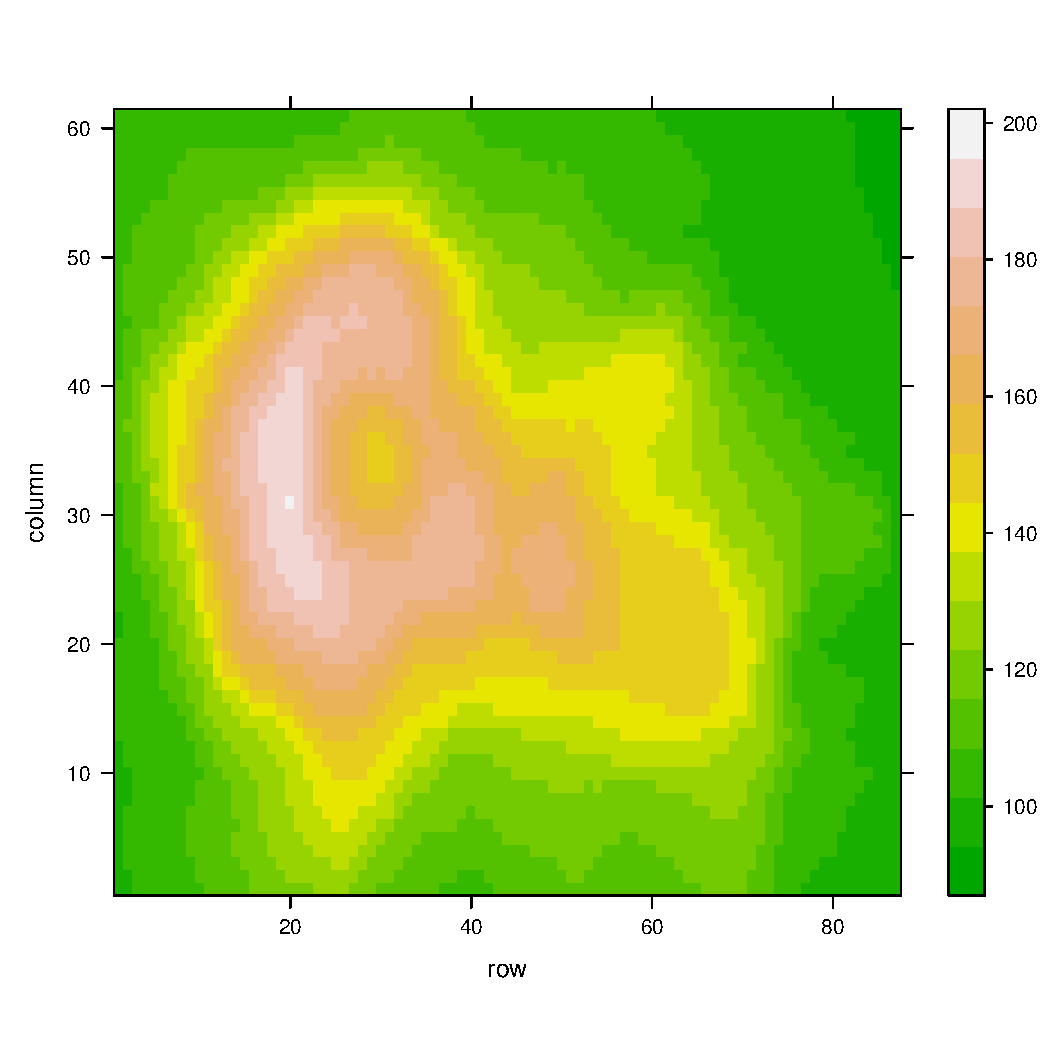
\includegraphics[width = 55mm]{images/levelplot.pdf}
\end{center}
\end{columns}
\end{frame}

%%%%%%%%%%%%%%%%%%%%%%%
\begin{frame}[fragile]
\frametitle{3D Images with Package \ttfamily lattice \normalfont}

\bf{Method 3:} \normalfont Same image with the \ttfamily image() \normalfont function:
    \begin{columns}
      \column{0.52\textwidth}
      
\begin{lstlisting}
x<-10*(1:nrow(volcano))
y<-10*(1:ncol(volcano))
image(x, y, volcano, col = terrain.colors(100), axes = TRUE)
contour(x, y, volcano, add = TRUE, col = 1)
\end{lstlisting}

     \column{0.48\textwidth}
       \begin{center}
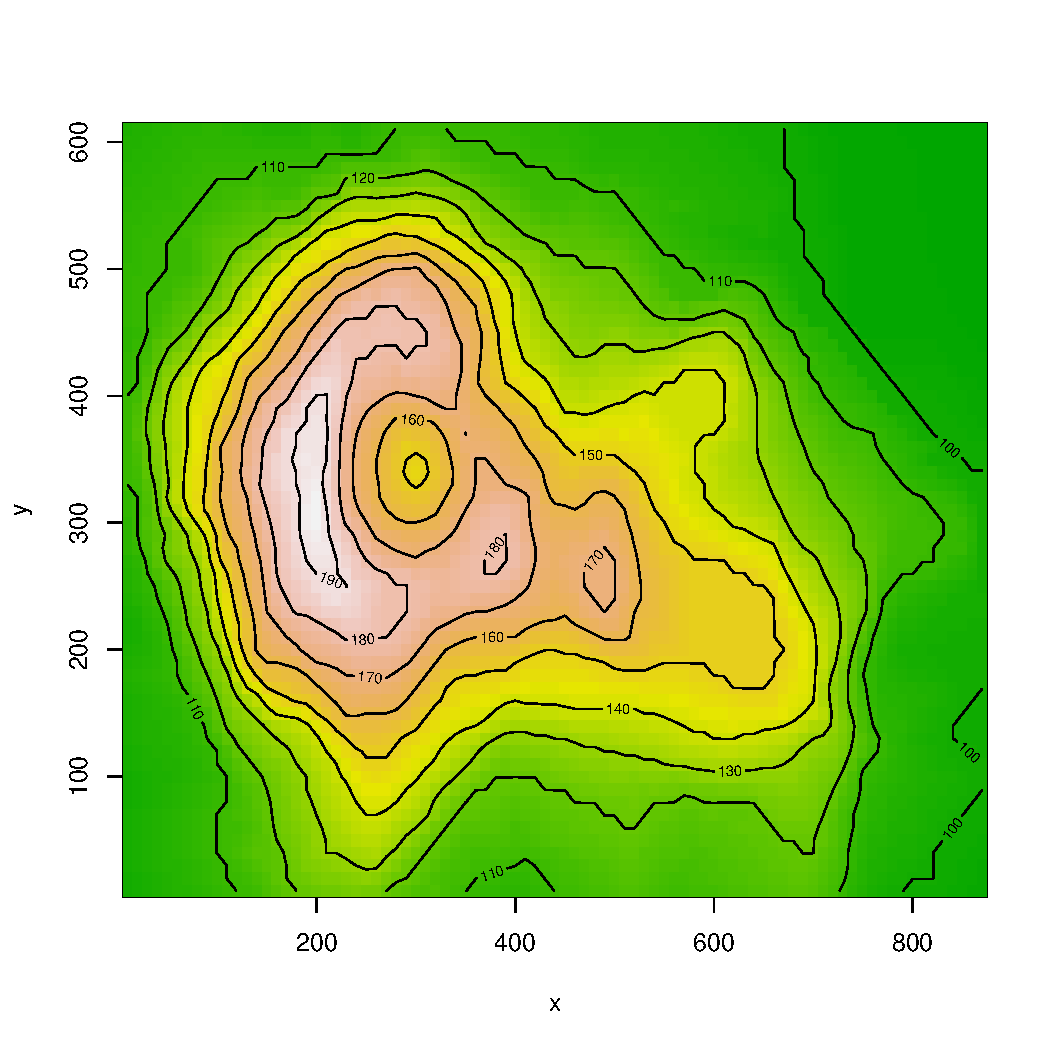
\includegraphics[width = 55mm]{images/image.pdf}
\end{center}
\end{columns}
\end{frame}
% plot3d(iris)

%%%%%%%%%%%%%%%%%%%%%%%
\subsection{\ttfamily ggplot2 \normalfont library} 
%%%%%%%%%%%%%%%%%%%%%%%
\begin{frame}[fragile, allowframebreaks]
\frametitle{3D Images with Package \ttfamily ggplot2 \normalfont}

Another way to create 3D images is with the package \ttfamily ggplot2: \normalfont 

%\bf{Method 1:} \normalfont Using \ttfamily wireframe(): \normalfont 
\begin{lstlisting}
# Step 1: Load the data
data(quakes)
attach(quakes)
# Step 2: Create a categorical variable for earthquake magnitude
ind<-which(mag<5)
ind2<-which(mag<6 & mag >=5)
ind3<-which(mag>=6)
color<-rep(NA, length(mag))
color[ind]<-1; color[ind2]<-2; color[ind3]<-3
color<-as.factor(color)


# Step 3: Plot
library(ggplot2)
ggplot(data=quakes, aes(long, lat))+
	geom_point(aes(long, lat))+
	borders("world")+
	coord_cartesian(xlim=c(100,190), ylim=c(-40,0))
\end{lstlisting}

\newpage
       \begin{center}
		\includegraphics[scale=0.22]{images/ggplotPlot1.pdf}
	\end{center}
\end{frame}

\begin{frame}[fragile, allowframebreaks]
\frametitle{3D Images with Package \ttfamily ggplot2 \normalfont}

To include information on magnitude of earthquake, use \ttfamily geom\_point(): \normalfont 

%\bf{Method 1:} \normalfont Using \ttfamily wireframe(): \normalfont 
\begin{lstlisting}
ggplot(data=quakes, aes(long, lat))+
	borders("world")+
	coord_cartesian(xlim=c(100,190), ylim=c(-40,0))+	
	geom_point(data=quakes, colour=as.numeric(color), size=2*as.numeric(color))
\end{lstlisting}

\newpage
       \begin{center}
		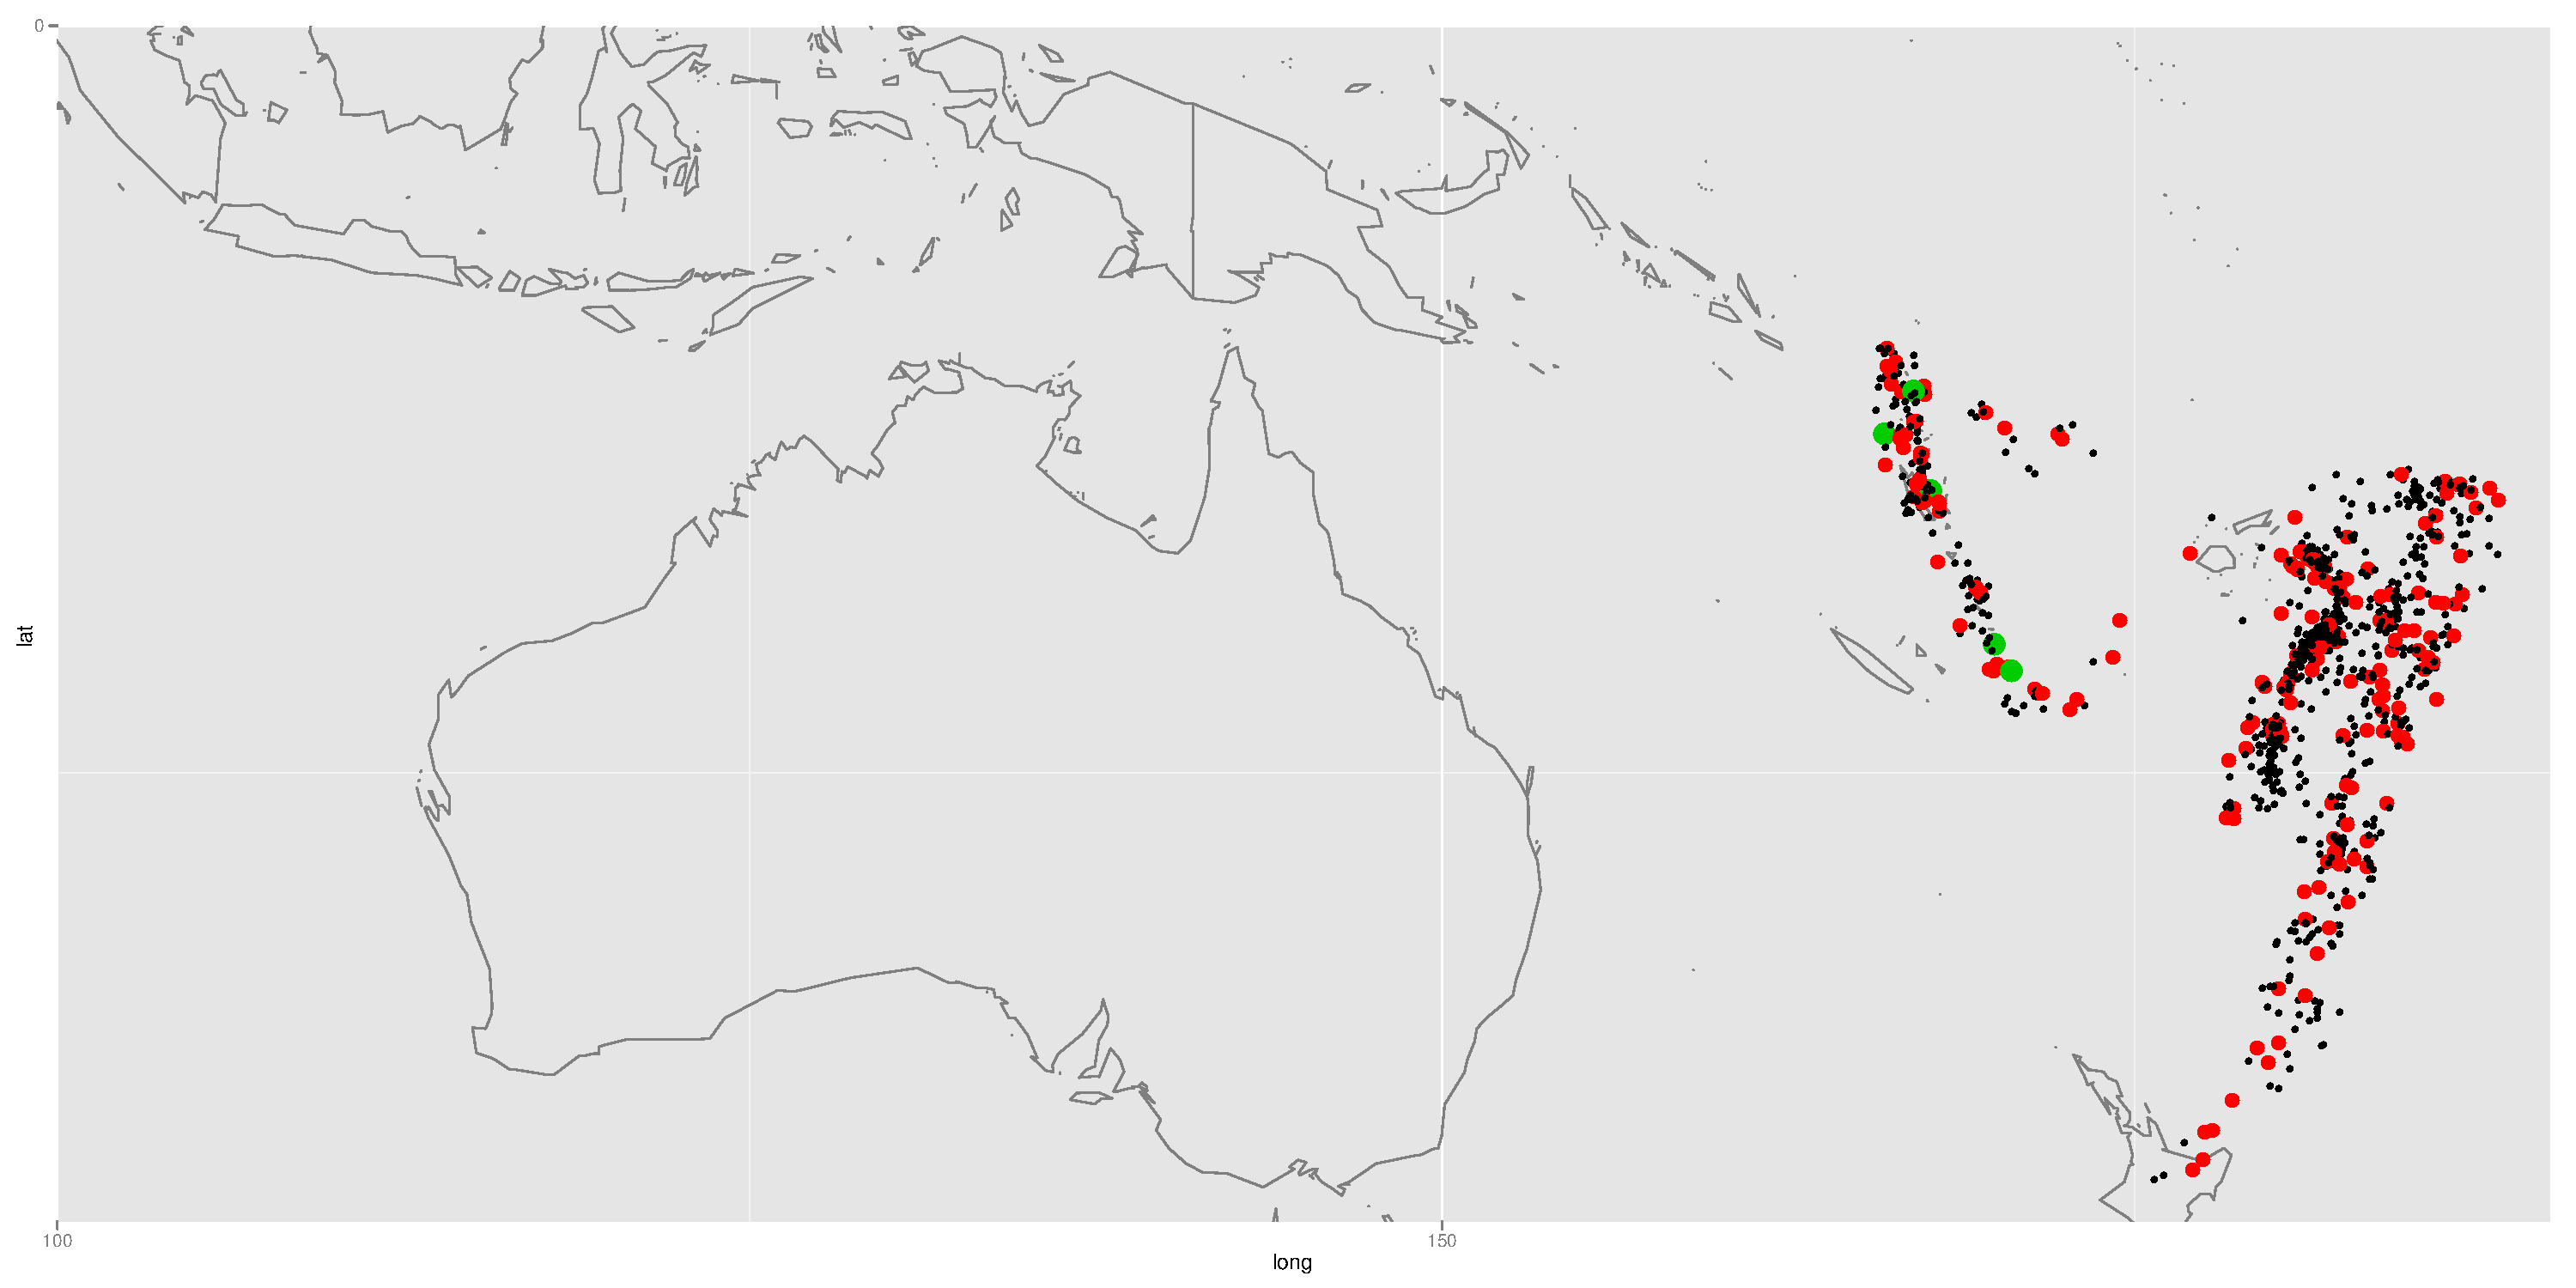
\includegraphics[scale=0.22]{images/ggplotPlot2.pdf}
	\end{center}
\end{frame}


%%%%%%%%%%%%%%%%%%%%%%%
\subsection{\ttfamily rgl \normalfont library} 
%%%%%%%%%%%%%%%%%%%%%%%
\begin{frame}[fragile]
\frametitle{3D Images with Package \ttfamily rgl \normalfont}

A way to create 3D interactive images is with the package \ttfamily rgl: \normalfont 

    \begin{columns}
      \column{0.50\textwidth}
\begin{lstlisting}
library(rgl)
data(quakes)
plot3d(x=quakes[, 2], y=quakes[, 1], z=quakes[, 3], xlab="Longitude", ylab="Latitude", zlab="Depth")
\end{lstlisting}
%g <- expand.grid(x = 1:10, y = 5:15)
%g$z<-g$x^2
%wireframe(g$z~g$x*g$y, scales = list(arrows = FALSE), drape = TRUE, colorkey = TRUE)

     \column{0.50\textwidth}
       \begin{center}
\includegraphics[width = 55mm]{images/Fiji_RGL}
\end{center}
\end{columns}
\end{frame}

%%%%%%%%%%%%%%%%%%%%%%%
\subsection{Saving Plots as a PDF} 
%%%%%%%%%%%%%%%%%%%%%%%
\begin{frame}[fragile]
\frametitle{Saving Plots as a PDF}
\framesubtitle{For Static Plots}

\itshape Note: \normalfont The files will be saved in the folder specified with \ttfamily setwd(). \normalfont
To save a static plot in \ttfamily R \normalfont as a PDF, use function \ttfamily pdf(): \normalfont

\begin{lstlisting}
# To save the image to the desktop:
setwd("~/Desktop")
wireframe(volcano, col.regions = terrain.colors(100), asp = 1, color.key=TRUE, drape=TRUE, scales = list(arrows = FALSE))
dev.off()
\end{lstlisting}

\end{frame}

\begin{frame}[fragile]
\frametitle{Saving Plots as a PDF}
\framesubtitle{For Dynamic Plots}

\itshape Note: \normalfont The files will be saved in the folder specified with \ttfamily setwd(). \normalfont
To save a dynamic plot in \ttfamily R \normalfont as a PDF, use function \ttfamily rgl.snapshot(): \normalfont

\begin{lstlisting}
# To save the image to the desktop:
setwd("~/Desktop")
# Step 1: Produce the 3D image:
plot3d(x=quakes[, 2], y=quakes[, 1], z=quakes[, 3], xlab="Longitude", ylab="Latitude", zlab="Depth")
# Step 2: Can rotate before taking a snapshot:
rgl.snapshot("quakes.png")
\end{lstlisting}

\end{frame}



% ------------------------------------------------------------
% ------------------------------------------------------------
\subsection{Exercise IV}
\begin{frame}
	\frametitle{Exercise IV}
	Use the \ttfamily rgl \normalfont library to create a 3D plot of the \ttfamily ozone \normalfont data set \footnote{\ttfamily http://www.ats.ucla.edu/stat/R/faq/ozone.csv\normalfont}.
\end{frame}		
		% lattice, plot3d ...
		% changing plotting options
		% contourplot, wireframe, levelplot
%	\section{Interactive Plots}

%%%%%%%%%%%%%%%%%%%%%%%
\subsection{\ttfamily rgl \normalfont library} 
%%%%%%%%%%%%%%%%%%%%%%%
\begin{frame}[fragile]
\frametitle{Dynamic visualizations with Package \ttfamily rgl \normalfont}

A way to create 3D interactive images is with the package \ttfamily rgl: \normalfont 

    \begin{columns}
      \column{0.55\textwidth}
\begin{lstlisting}[ basicstyle=\footnotesize ]
library(rgl)
data(quakes)
plot3d(
	x=quakes$long, 
	y=quakes$lat, 
	z=quakes$depth, 
	xlab="Longitude", 
	ylab="Latitude", 
	zlab="Depth"
	)
\end{lstlisting}
%g <- expand.grid(x = 1:10, y = 5:15)
%g$z<-g$x^2
%wireframe(g$z~g$x*g$y, scales = list(arrows = FALSE), drape = TRUE, colorkey = TRUE)

     \column{0.45\textwidth}
       \begin{center}
\includegraphics[width = 55mm]{images/Fiji_RGL}
\end{center}
\end{columns}
\end{frame}

%------------------------------------
\subsection{\ttfamily ??? \normalfont library} 
%------------------------------------
\begin{frame}[fragile]
	\frametitleDynamic Visualizations with Package \ttfamily ??? \normalfont}
\end{frame}

%------------------------------------
\subsection{\ttfamily shiny \normalfont library} 
\begin{frame}[fragile]
	\frametitle{Interactive visualizations with Package \ttfamily shiny \normalfont}
\end{frame}
%------------------------------------

% ------------------------------------------------------------
% ------------------------------------------------------------
\subsection{Exercise IV}
\begin{frame}
	\frametitle{Exercise IV}
	Use the \ttfamily rgl \normalfont library to create a 3D plot of the \ttfamily ozone \normalfont data set \footnote{\ttfamily http://www.ats.ucla.edu/stat/R/faq/ozone.csv\normalfont}.
\end{frame}			
	%
% ------------------------------------------------------------
% ------------------------------------------------------------

%%%%%%%%%%%%%%%%%%%%%%%%%%%%%%%%%%%%%
\section{Simulations}
\begin{frame}[fragile]
\frametitle{Simulations I}
\framesubtitle{Preliminaries: The function \ttfamily outer() \normalfont}

    \begin{columns}[Tc]
      \column{0.42\textwidth}
\begin{lstlisting}
x=5:6; y=1:3
outer(x,y)
\end{lstlisting}

\begin{beamerboxesrounded}[shadow=true]{}
\ttfamily
\begin{verbatim}
     [,1] [,2] [,3] 
[1,]    5   10   15 
[2,]    6   12   18 
\end{verbatim}
\end{beamerboxesrounded}
\normalfont

	     \column{0.58\textwidth}
\begin{lstlisting}
fcn<-function(x,y){z=x+y}
outer(x,y,fcn)
\end{lstlisting}

\begin{beamerboxesrounded}[shadow=true]{}
\ttfamily
\begin{verbatim}
     [,1] [,2] [,3] 
[1,]    6    7    8 
[2,]    7    8    9 
\end{verbatim}
\end{beamerboxesrounded}
\normalfont
	\end{columns}
\end{frame}

%%%%%%%%%%%%%%%%%%%
\begin{frame}[fragile]
\frametitle{Simulations II}
Suppose we want to know what the function $y\times sin(x)$ looks like:

\begin{lstlisting}
# Sample from the random uniform:
x <- sort(runif(100, min=0, max=10))
y <- x+runif(1)
f <- function(x,y) { r <- y*sin(x)}
z <- outer(x,y,f)
persp(x, y, z, col = "lightblue", shade = 0.1, ticktype = "detailed", expand=0.7)
\end{lstlisting}
\end{frame}

\begin{frame}[fragile]
\frametitle{Simulations III}
   \begin{figure}[ht]
       \begin{center}
		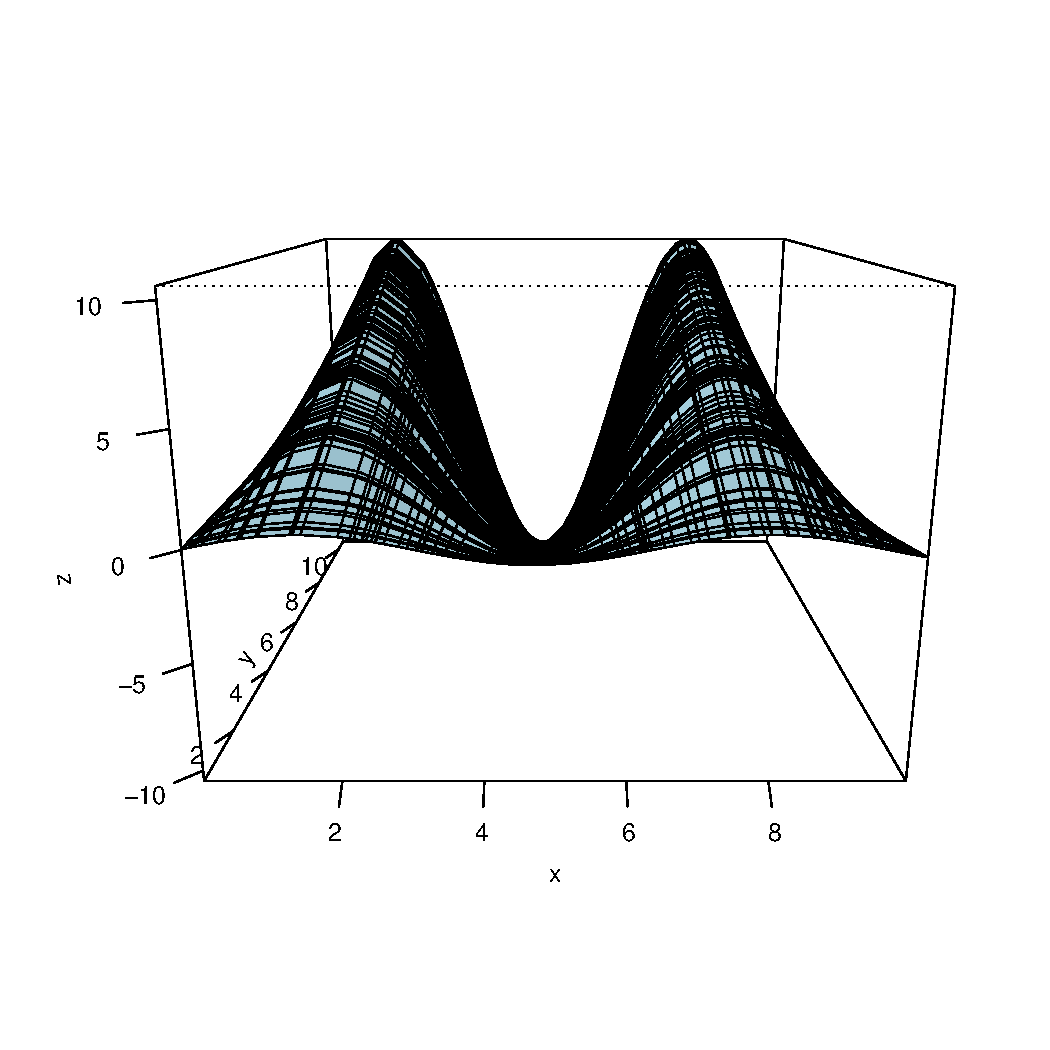
\includegraphics[width = 3.5in]{images/simulation.png}
	\end{center}
   \end{figure}
\end{frame}

\begin{frame}[fragile]
\frametitle{Simulations IV}
To visually see its maximum and minimum values, look at the contours of the function:

    \begin{columns}[Tc]
      \column{0.36\textwidth}

\begin{lstlisting}
contour(x,y,z)
\end{lstlisting}

     \column{0.64\textwidth}
   \begin{figure}[ht]
       \begin{center}
		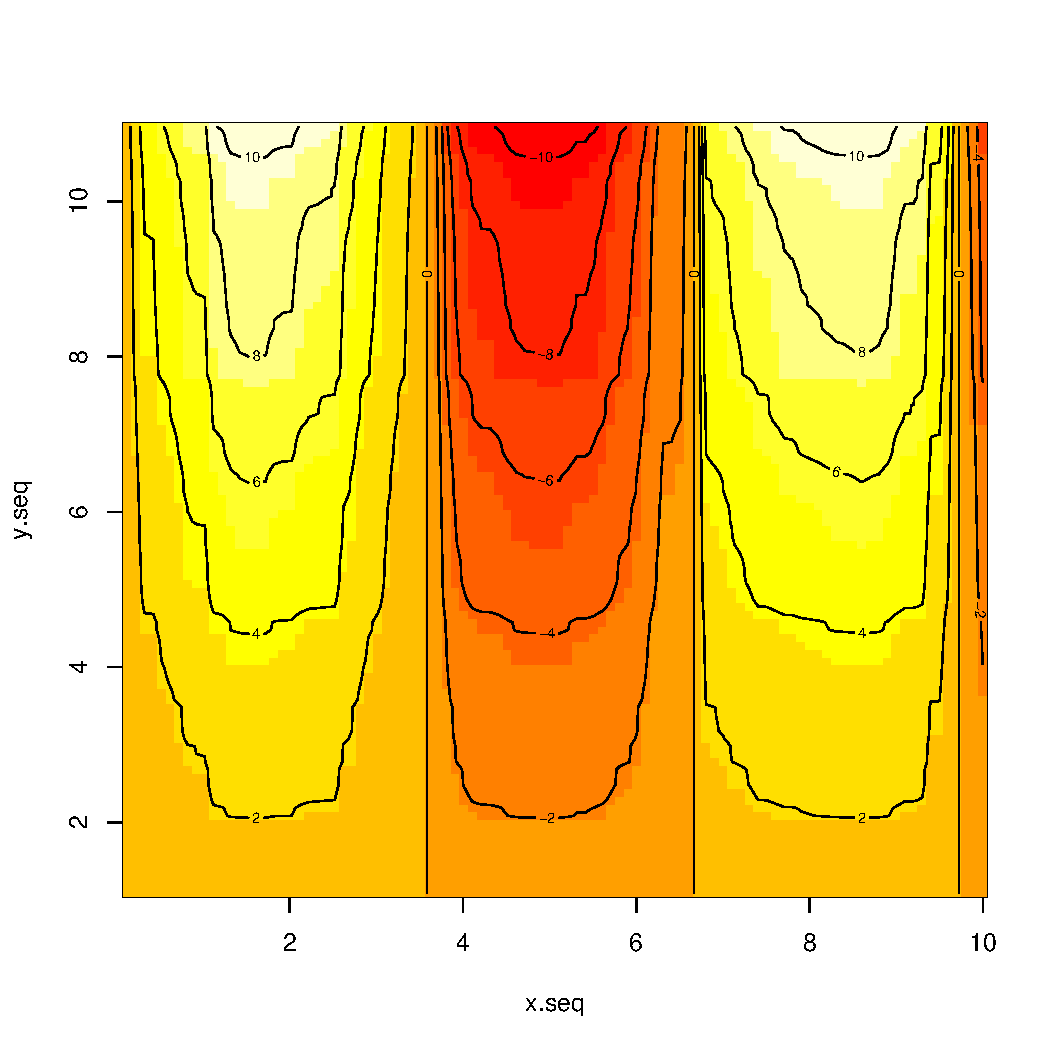
\includegraphics[scale=0.33]{images/contourSim.pdf}
	\end{center}
   \end{figure}
\end{columns}

\end{frame}


%g <- expand.grid(x = 1:10, y = 5:15)
%g$z<-g$x^2
%wireframe(g$z~g$x*g$y, scales = list(arrows = FALSE), drape = TRUE, colorkey = TRUE)


% ------------------------------------------------------------
% ------------------------------------------------------------

		% see 202C R Code		
	%%%%%%%%%%%%%%%%%% Section: Exercise
\section[Solutions]{Solutions to the Exercises}
%_______________________ Subsection
  \subsection{Solution to Exercise I}
\begin{frame}[fragile]
  \frametitle{Solution to Exercise I}

			\begin{lstlisting}
beanplot(Sepal.Width ~ Species, data=iris, col=list(grey(0.5),c(grey(0.8),"white")), border = NA, overallline = "median", ll=0.01, side="both")
			\end{lstlisting}
\end{frame}

%_______________________ Subsection
  \subsection{Solution to Exercise II}
  \begin{frame}[fragile]
  \frametitle{Solution to Exercise II}

			\begin{lstlisting}
source("http://www.biostat.jhsph.edu/~rpeng/RR/mvtsplot/mvtsplot.R")		
mvtsplot(EuStockMarkets)
			\end{lstlisting}
\end{frame}

%_______________________ Subsection
  \subsection{Solution to Exercise III}
\begin{frame}[fragile]
  \frametitle{Solution to Exercise III}

			\begin{lstlisting}
ozone<-read.table("http://www.ats.ucla.edu/stat/R/faq/ozone.csv", sep=",", header=T)
attach(ozone)
plot(Lat~Lon, xlim=c(-125, -113), ylim=c(31,42))
map("state", "california", add=TRUE)
			\end{lstlisting}

\end{frame}

%_______________________ Subsection
\subsection{Solution to Exercise IV}
  \begin{frame}[fragile]
  \frametitle{Solution to Exercise IV}
 		\begin{lstlisting}
ozone<-read.table("http://www.ats.ucla.edu/stat/R/faq/ozone.csv", sep=",", header=T)
attach(ozone)
library(rgl)
plot3d(z=Av8top, x=long, y=lat)
 		\end{lstlisting}
\end{frame}

%_______________________ Subsection
\subsection{Solution to Exercise V}
  \begin{frame}[fragile]
  \frametitle{Solution to Exercise V}
 		\begin{lstlisting}
# Sample from the random uniform:
x <- sort(runif(100, min=0, max=10))
y <- x+runif(1)
f <- function(x,y) { r <- sin(1.5*x)/y}
z <- outer(x,y,f)
persp(x, y, z, col = terrain.colors(length(z)/4), shade = 0.1, ticktype = "detailed", expand=0.7)
 		\end{lstlisting}
\end{frame}

	% ------------------------------------------------------------
%%%%%%%%%%%%%%%%% Online Resources
\section[Links]{Useful Links for R}
\begin{frame}[fragile]
  \frametitle{Online Resources for R}
%\begin{description}[<+->] 
%\item[Download R:] http://cran.stat.ucla.edu/
%\item[Search Engine for R:] http://rseek.org
%\item[R Reference Card:] http://cran.r-project.org/doc/contrib/Short-refcard.pdf
%\item[UCLA Statistics Information Portal:] http://info.stat.ucla.edu/grad/
%\item[UCLA Statistical Consulting Center:] http://scc.stat.ucla.edu
%\end{description}

\begin{description}
	\item[Download R:] {\small \textit{\urlwofont{http://cran.stat.ucla.edu/}}}
	\item[Search Engine for R:] {\small \textit{\urlwofont{http://rseek.org}}}
	\item[R Reference Card:] $\:$ \\
		{\small \textit{\urlwofont{http://cran.r-project.org/doc/contrib/Short-refcard.pdf}}}
	\item[R Graphics Gallery:] $\:$ \\
		 {\small \textit{\urlwofont{http://research.stowers-institute.org/efg/R/}}}
	\item [R Graph Gallery:]  {\small \textit{\urlwofont{http://addictedtor.free.fr/graphiques/}}}
	\item[UCLA Statistics Information Portal:] \small{ \textit{\urlwofont{http://info.stat.ucla.edu/grad/}}}
	\item[UCLA Statistical Consulting Center:] \small{ \textit{\urlwofont{http://scc.stat.ucla.edu}}}
\end{description}
\end{frame}
%_________________________________ Part
%%%%%%%%%%%%%%%%%% Section: Exercise

%\frame{
%  \frametitle{Upcoming Mini-Course}
%	\framesubtitle{This Wednesday}
%$4:30$PM: Advanced Graphics with \ttfamily R \normalfont
%}

\frame{
  \frametitle{}
\begin{center}
Thank you.\\

Any questions?
\end{center}
}

	
%>     -histograms (and overlaying sample and normal densities to it)
%>     -boxplots and adding details
%>     -points plots with different characters and options
%>     -overlaying maps
%>     -creating bubbleplots
%>     -lattice graphics
%>     -3D graphics: scatterplot3d and plot3d
%>     -formatting plots
%>     -saving plots as PDFs, BMP, etc
%>     -creating tables (to be used in LaTeX)
%	
\end{document}

%%% Cartoons to add:
% http://xkcd.com/1048/
% http://xkcd.com/668/
% https://xkcd.com/688/
% http://xkcd.com/1138/
% https://xkcd.com/833/
% http://xkcd.com/795/
%%% Create the most popular visuals in R:
% map
% stack graph



%%% TODO:
% - facebook blog/pic: https://www.facebook.com/notes/facebook-engineering/visualizing-friendships/469716398919
% - geographic with cholropleth or shapefiles: 
%		- http://www.kevjohnson.org/making-maps-in-r/
%		- http://spatialdemography.org/wp-content/uploads/2013/04/9.-Sparks.pdf
%		- http://zevross.com/blog/2015/10/14/manipulating-and-mapping-us-census-data-in-r-using-the-acs-tigris-and-leaflet-packages-3/
% - sankey via rCharts: http://www.r-bloggers.com/generating-sankey-diagrams-from-rcharts/
% - shiny
% - leaflet: 
%		- http://www.r-bloggers.com/building-interactive-maps-with-leaflet/
%		- http://robinlovelace.net/r/2015/02/01/leaflet-r-package.html
% - nodes with directed edges
%%%
% - where to go from here: subsetting, functions, visualizations and http://statacumen.com/teach/SC1/SC1_18_Plots.pdf

% LA county shapefiles: http://www.census.gov/geo/partnerships/pvs/partnership15v2/st06_ca.html
% CA shapefiles: https://www.census.gov/geo/maps-data/data/cbf/cbf_tracts.html
% http://www.r-bloggers.com/a-tall-drink-of-water/?utm_source=feedburner&utm_medium=email&utm_campaign=Feed%3A+RBloggers+%28R+bloggers%29

% Yelp data: https://www.kaggle.com/c/yelp-recruiting

% Get data for CA hospitals: https://chhs.data.ca.gov/Healthcare/Number-of-Selected-Inpatient-Medical-Procedures-Ca/mdt8-gwyw


% subsetting fcn
